\subsection{A deblending test}
\label{sec:deblending_test}

In this section we demonstrate the performance of StarNet on deblending two stars. Two stars were simulated in an $7\times 7$ image. The input to StarNet was the entire $7\times 7$ image; no tiling was used in this expeirment. 
We trained StarNet using the sleep phase, with prior described in Section~\ref{sec:gen_model}, except that the number of stars was uniform: with equal probability, there is either 0, 1, or 2 stars in the image. 

Figure~\ref{fig:deblending_test} displays the probability that $N = 2$ under our variational posterior, as the distance between two stars varies.
As the flux increases, stars become easier to deblend.
As the difference in flux between the two stars increases, the stars become harder to deblend. 
Finally, color differences between the stars aid in their deblending.

\begin{figure}[!h]
    \centering
    \begin{subfigure}{0.95\textwidth}
        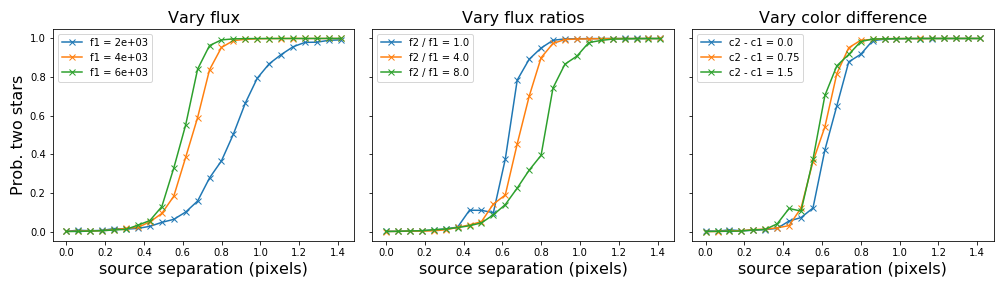
\includegraphics[width=\textwidth]{figures/deblending_test.png}
    \end{subfigure}
      \begin{subfigure}{0.95\textwidth}
        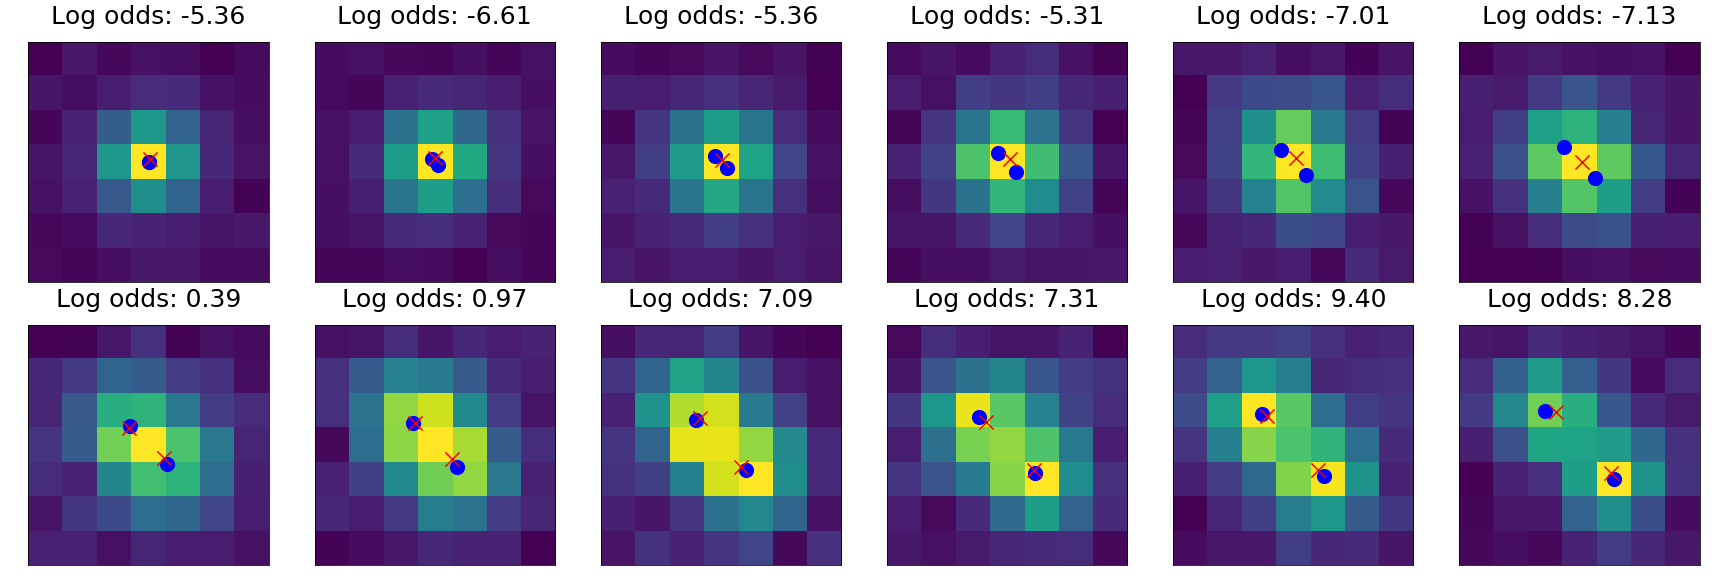
\includegraphics[width=\textwidth]{figures/deblending_ex_test.png}
    \end{subfigure}
    \label{fig:deblending_test}
    \caption{(Top row) The probability under $q$ that the image region constains two stars as source separation increases.
    On the left, both stars have the same flux, and their common flux was varied. In the middle, both stars have color = 0, and the first star had flux = 4000. We varied the flux of the second star to have the same, four times, or eight times the flux of the first star. On the right, both stars have $r$-band flux = 4000; the color of the first star is 0. The color of the second star was varied.
    (Bottom) An example of detections as source separation increases. Red are MAP detections, blue are true locations. Log odds are probability of two stars over probability of one star. Here, both stars have flux = 4000 and color = 0.}
    \label{fig:sparse_field}
\end{figure}
